%%%%%%%%%%%%%%%%%%%%%%%%%%%%%%%%%%%%%%%%%
% Beamer Presentation
% LaTeX Template

\documentclass{beamer}
\mode<presentation> {
\usetheme{Warsaw}
}

\usepackage{multicol}
\usepackage[russian]{babel}
\usepackage{graphicx} 
\usepackage{hyperref}

\title[Introduction to Python]{Glimpse into Machine learning} 
\author{Sugarkhuu Radnaa} 
\institute[]
{
Py4Econ in Ulaanbaatar \\ 
\medskip
\textit{py4econ@gmail.com} 
}
\date{\today}  % 

\begin{document}

\begin{frame}
\titlepage % Print the title page as the first slide
\end{frame}

\begin{frame}
    \frametitle{Week 8: Learning objectives}
    \begin{itemize}
        \item Prerequisites for Machine learning 
        \item Machine learning workflow
        \item Machine learning versus Deep learning|AI
        \item Different types of Machine learning algorithms
    \end{itemize}
\end{frame}

% %------------------------------------------------
% \section{Different file types} 
% %------------------------------------------------

\begin{frame}
    \frametitle{Prerequisites for Machine learning}
            \begin{itemize}
                \item Algebra and linear algebra (Matrix)
                \item Probability and statistics
                \item Calculus (derivaties)
                \item Programming language (Python, R, C++, Matlab)
                \item Terminal (shell)                
            \end{itemize}
\end{frame}

\begin{frame}
    \frametitle{Machine learning pipeline 1}
    \begin{center}
        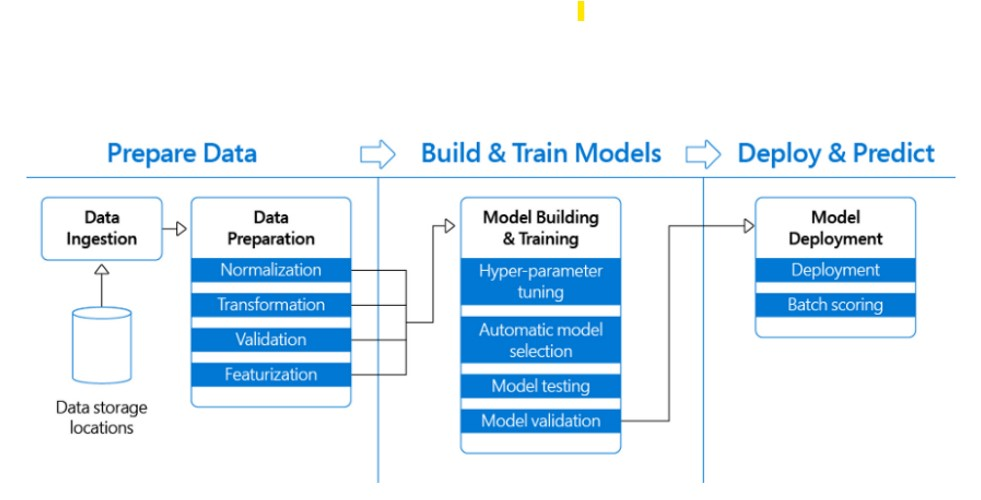
\includegraphics[scale=0.5]{figures/ML_pipe.jpg}
    \end{center}
\end{frame}

\begin{frame}
    \frametitle{Machine learning pipeline 2}
    \begin{center}
        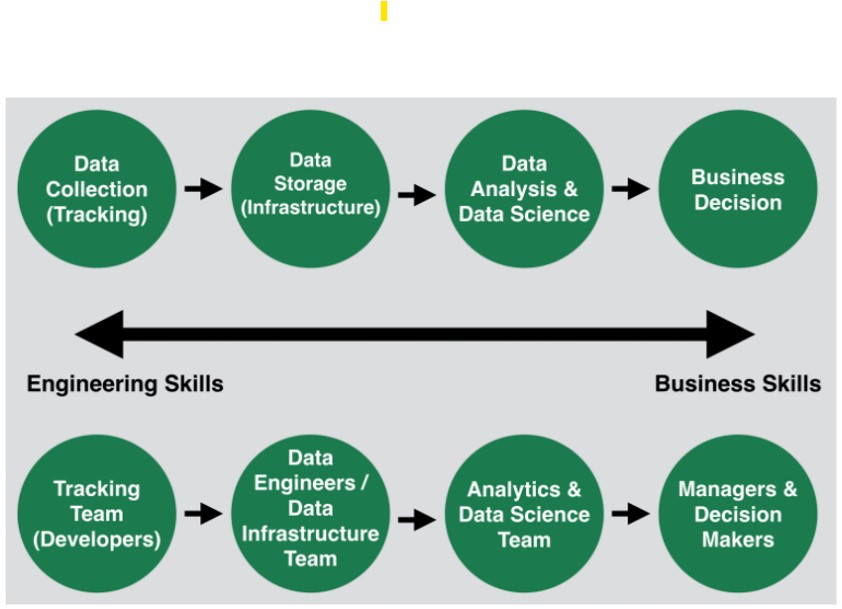
\includegraphics[scale=0.5]{figures/ML_pipe_2.jpg}
    \end{center}
\end{frame}

\begin{frame}
    \frametitle{Machine learning in bigger scope}
    \begin{center}
        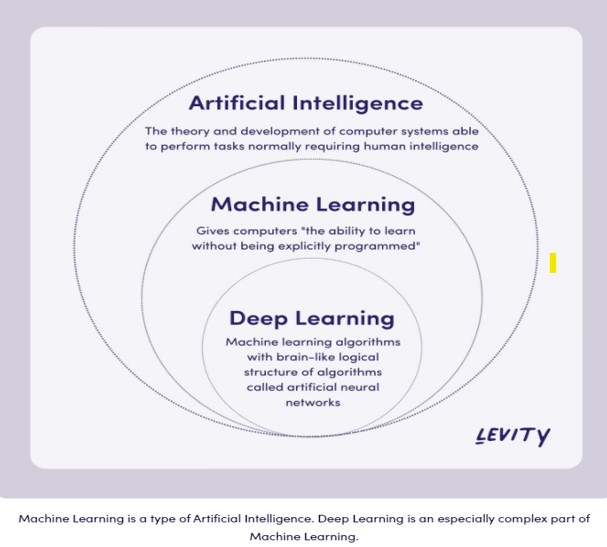
\includegraphics[scale=0.5]{figures/ml_in_ai.jpg}
    \end{center}
\end{frame}

\begin{frame}
    \frametitle{Machine learning versus deep learning}
    \begin{center}
        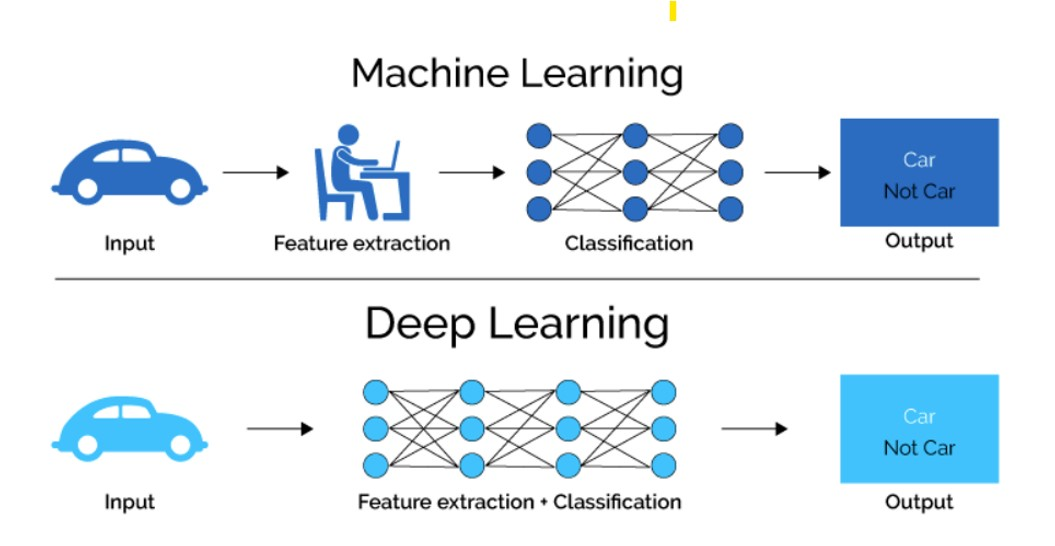
\includegraphics[scale=0.5]{figures/ml_vs_deep.jpg}
    \end{center}
\end{frame}

\begin{frame}
    \frametitle{Different machine learning algorithms}
    \begin{center}
        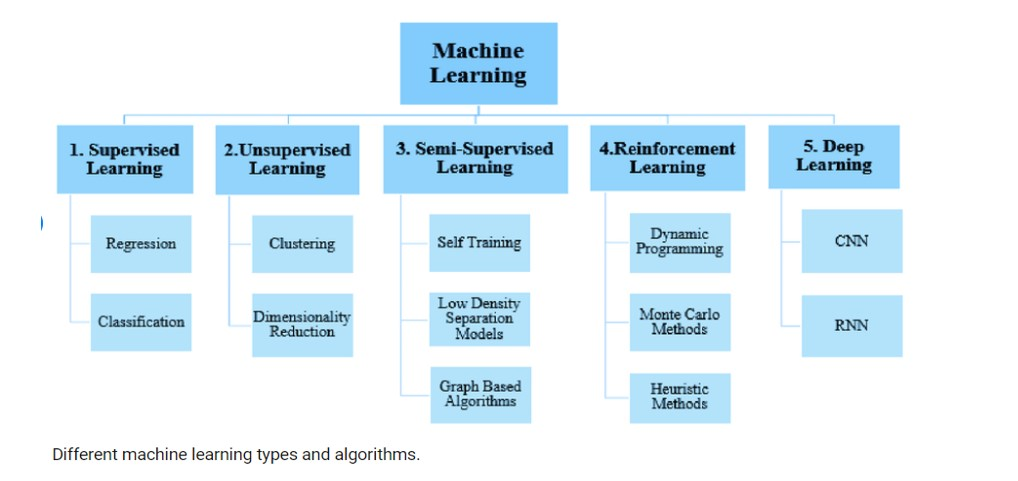
\includegraphics[scale=0.5]{figures/ml_types.jpg}
    \end{center}
\end{frame}

\begin{frame}
    \frametitle{Sample machine learning projects}
    \begin{itemize}
        \item \url{https://www.kaggle.com/dansbecker/your-first-machine-learning-model/tutorial}
        \item \url{https://www.kaggle.com/kanncaa1/machine-learning-tutorial-for-beginners#DATA-SCIENTIST}
        \item \url{https://jakevdp.github.io/PythonDataScienceHandbook/}
        \item \url{https://github.com/EthicalML/awesome-production-machine-learning}
        \item \url{https://www.analyticsvidhya.com/blog/2020/09/integrating-machine-learning-into-web-applications-with-flask/}
        \begin{itemize}
            \tiny
            \item \url{https://github.com/NakulLakhotia/deploheroku}
            \item \url{https://ml-with-flask.herokuapp.com/}
        \end{itemize} 
    \end{itemize}
\end{frame}

%------------------------------------------------
\section{Homework} 
%------------------------------------------------

\begin{frame}
    \frametitle{Project 3}
\vskip 2mm
Deadline: 31 January, 2022 \\

\vfill
\textbf{Note:} Create a github repo from the start and populate it with your results
\end{frame}

\begin{frame}
    \frametitle{Dashboard}
    Project 1 дэх өгөгдөл болон түүний түүхэн өгөгдлүүдийг ашиглан Bokeh dashboard үүсгэнэ үү. 

    Жишээ: 

    \begin{itemize}
        \item \url{https://github.com/bokeh/bokeh/tree/branch-3.0/examples/app/dash}
    \end{itemize}
\end{frame}


\begin{frame}
\Huge{\centerline{Thank you!}}
\end{frame}

%----------------------------------------------------------------------------------------

\end{document} 